\begin{figure}[t]
{\centering
\begin{minipage}{0.48\textwidth}
  \footnotesize
  \centering
  \begin{tabular}{@{}l@{}rr@{}l@{}rr@{}}
    \toprule
    & \multicolumn{2}{c}{CNN} &\phantom{aa}& \multicolumn{2}{c}{Daily Mail} \\
    \cmidrule{2-3} \cmidrule{5-6}
    & valid & test && valid & test \\
    \midrule
    Maximum frequency              & 30.5 & 33.2 && 25.6 & 25.5 \\
    Exclusive frequency            & 36.6 & 39.3 && 32.7 & 32.8 \\
    Frame-semantic model~~         & 36.3 & 40.2 && 35.5 & 35.5 \\
    Word distance model            & 50.5 & 50.9 && 56.4 & 55.5 \\
    \midrule
    Deep LSTM Reader               & 55.0 & 57.0 && 63.3 & 62.2 \\
    Uniform Reader                 & 39.0 & 39.4 && 34.6 & 34.4 \\
    Attentive Reader               & 61.6 & 63.0 && {\bf 70.5} & {\bf 69.0} \\
    Impatient Reader               & {\bf 61.8} & {\bf 63.8} && 69.0 & 68.0 \\
    \bottomrule
  \end{tabular}
  \captionof{table}{Accuracy of all the models and benchmarks on the CNN and
                    Daily Mail datasets.
                    The Uniform Reader baseline sets all of the $m(t)$
                    parameters to be equal.}
  \label{tab:main_results}
\end{minipage}
\hspace{0.15in}
\begin{minipage}{0.47\textwidth}
\centering
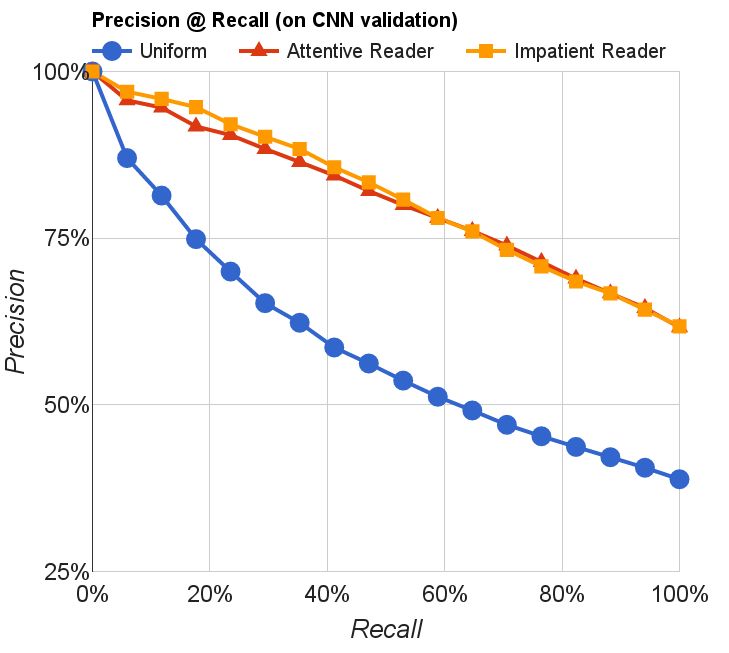
\includegraphics[scale=0.24,trim=0 0.3cm 0 1.3cm,clip=true]{{figs/patrcnnnew}.png}\\[-0.3em]
\captionof{figure}{Precision@Recall for the attention models on the CNN validation data.}
\label{fig:patr}
\end{minipage}
}
\end{figure}


\paragraph{Frame-semantic benchmark}

While the one frame-semantic model proposed in this paper is clearly a
simplification of what could be achieved with annotations from an NLP pipeline,
it does highlight the difficulty of the task when approached from a symbolic NLP
perspective.

Two issues stand out when analysing the results in detail. First, the
frame-semantic pipeline has a poor degree of coverage with many relations not
being picked up by our PropBank parser as they do not adhere to the default
predicate-argument structure. This effect is exacerbated by the type of language
used in the highlights that form the basis of our datasets.
The second issue is that the frame-semantic approach does not trivially scale to
situations where several sentences, and thus frames, are required to answer a
query. This was true for the majority of queries in the dataset.


\paragraph{Word distance benchmark}

More surprising perhaps is the relatively strong performance of the word
distance benchmark, particularly relative to the frame-semantic benchmark, which
we had expected to perform better. Here, again, the nature of the datasets used
can explain aspects of this result. Where the frame-semantic model suffered due
to the language used in the highlights, the word distance model benefited.
Particularly in the case of the Daily Mail dataset, highlights frequently have
significant lexical overlap with passages in the accompanying article,
which makes it easy for the word distance benchmark.
For instance the query ``\textit{Tom Hanks is friends with {\bf X}'s
manager, Scooter Brown}'' has the phrase ``\textit{... turns out he is good
friends with Scooter Brown, manager for Carly Rae Jepson}'' in the context. The
word distance benchmark correctly aligns these two while the frame-semantic
approach fails to pickup the friendship or management relations when parsing
the query.
We expect that on other types of machine reading data where questions rather
than Cloze queries are used this particular model would perform significantly
worse.


\paragraph{Neural models}

Within the group of neural models explored here, the results paint a clear
picture with the Impatient and the Attentive Readers outperforming all other
models. This is consistent with our hypothesis that attention is a key
ingredient for machine reading and question answering due to the need to
propagate information over long distances.  The Deep LSTM Reader
performs surprisingly well, once again demonstrating that this simple sequential
architecture can do a reasonable job of learning to abstract long sequences,
even when they are up to two thousand tokens in length.  However this model does
fail to match the performance of the attention based models, even though these
only use single layer LSTMs.\footnote{Memory constraints prevented us from
experimenting with deeper Attentive Readers.}

The poor results of the Uniform Reader support our hypothesis of
the significance of the attention mechanism in the Attentive model's
performance as the only difference between these models is that the attention
variables are ignored in the Uniform Reader. The precision@recall statistics in
Figure~\ref{fig:patr} again highlight the strength of the attentive approach.

We can visualise the attention mechanism as a heatmap over a context document to
gain further insight into the models' performance. The highlighted words show
which tokens in the document were attended to by the model. In addition we must
also take into account that the vectors at each token integrate long range
contextual information via the bidirectional LSTM encoders.
Figure \ref{fig:heatmaps} depicts heat maps for two queries that were correctly
answered by the Attentive Reader.\footnote{Note that these examples were chosen
as they were short, the average CNN validation document contained 763 tokens and
27 entities, thus most instances were significantly harder to answer than these
examples.} In both cases confidently arriving at the correct answer requires the
model to perform both significant lexical generalsiation, e.g.\ `killed'
$\rightarrow$ `deceased', and co-reference or anaphora resolution, e.g.\
`{\em ent119} was killed' $\rightarrow$ `he was identified.' However it is also
clear that the model is able to integrate these signals with rough heuristic
indicators such as the proximity of query words to the candidate answer.

\begin{figure}[t]
  \centering
  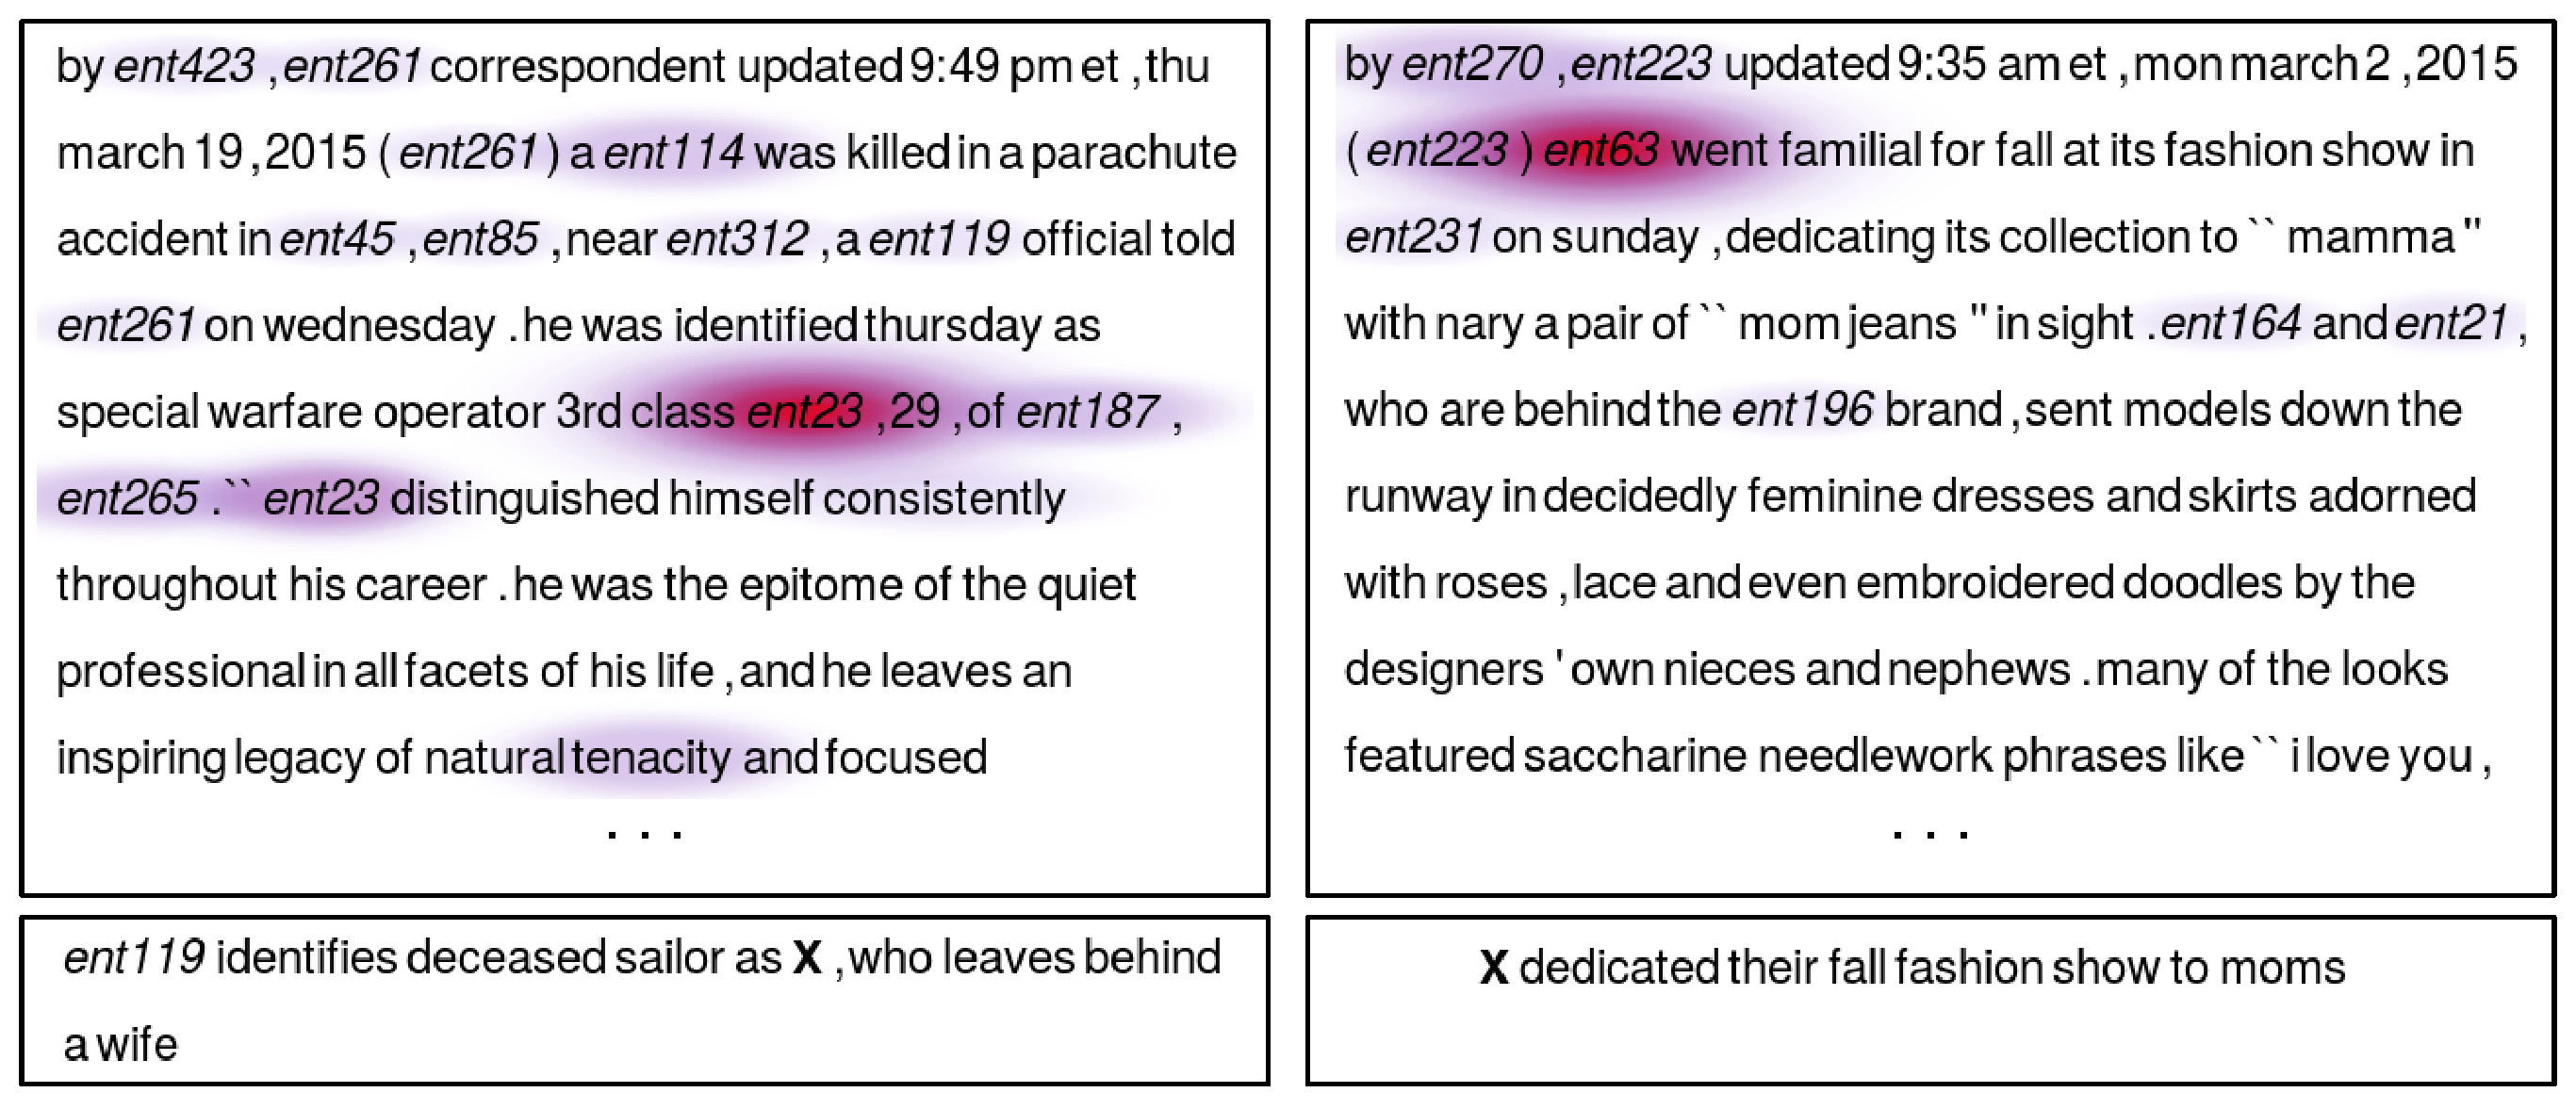
\includegraphics[scale=0.30]{{figs/pairOfExampleHeatmaps}.pdf}
  \caption{Attention heat maps from the Attentive Reader for two
    correctly answered validation set queries (the correct answers are
    \textit{ent23} and \textit{ent63}, respectively). Both examples
           require significant lexical generalisation and co-reference
           resolution in order to be answered correctly by a given model.}
  \label{fig:heatmaps}
\end{figure}


